\section{La forêt aléatoire}
\label{chap4.section3}
La forêt aléatoire est un algorithme de classification basé sur les arbres de décisions. Un aspect importants des arbres de décisions et des modèles non paramétriques en général est que ce sont les modèles les plus sensibles au sur-ajustement\footnote{Le sur-ajustement est le nom du phénomène qui se produit quand un modèle d'apprentissage n'arrive pas à généraliser mais excelle à prédire les données d'entraînement. C'est un signe que le modèle est trop dépendant de la structure et des exemples de l'ensemble d'entraînement, on dit donc qu'il est sur-ajuster sur les données d'entraîment} ou \textbf{overfitting}. Comme son nom laisse entendre, l'idée derrière l'algorithme de la forêt aléatoire de est de combiner ou de sommer les prédictions de plusieurs arbres de décisions entraînés sur différents sous groupes (créés aléatoirement) de l'ensemble d'entraînement (\cite{breiman2001random}). C'est la philosophie des \textbf{techniques d'ensemble} de \textit{Bagging} qui cherche à combiner ou confronter les prédictions de plusieurs apprenants faibles ou \textbf{weak learners} (traditionnellement des arbres de décisions) en espérant que leur divergence corrige leur bias respectifs. Cela resulte en des modèles moins sensible au sur-ajustement et donc une meilleur capacité de généralisation puisque la classification ne dépend plus seulement d'un arbre potentiellement sur-ajusté mais de toute une forêt avec des individus de différents schéma, perception et bias.

\subsection{Algorithme}
\label{chap4.sec3.sub1}
Bien que les implémentations peuvent différer, l'algorithme général se présente comme suit:

\begin{enumerate}
    \item \textbf{Créer des sous-ensemble}: Diviser l'ensemble d'entraînment en sous ensemble de manière aléatoire et avec répétition (c'est-à-dire que des exemples peuvent être répété dans différent sous-ensemble). Les différents sous ensemble peuvent être de même taille ou pas.
    \item \textbf{Entraîner les arbres de décisions}: Entraîner un arbre de décision sur chaque sous-ensemble en utilisant l'algorithme décrit dans la section \ref{chap4.sec2.sub3}
    \item \textbf{Prediction}: Pour l'ensemble de test, combiner les prédictions des arbres entraînés lors de l'étape 2. Traditionnellemnt on performe un vote entre les arbres de la forêt, c'est-à-dire que l'étiquette le plus prédite est choisi comme prédiction de la forêt mais on peut aussi appliquer n'importe quelle fonction de sommation, par exemple l'algorithme pourrait retourner la probabilité de chaque classe.
\end{enumerate}

Une illustration de cet algorithme est montré dans la figure \ref{fig:fig5}

\begin{figure}
    \centering
    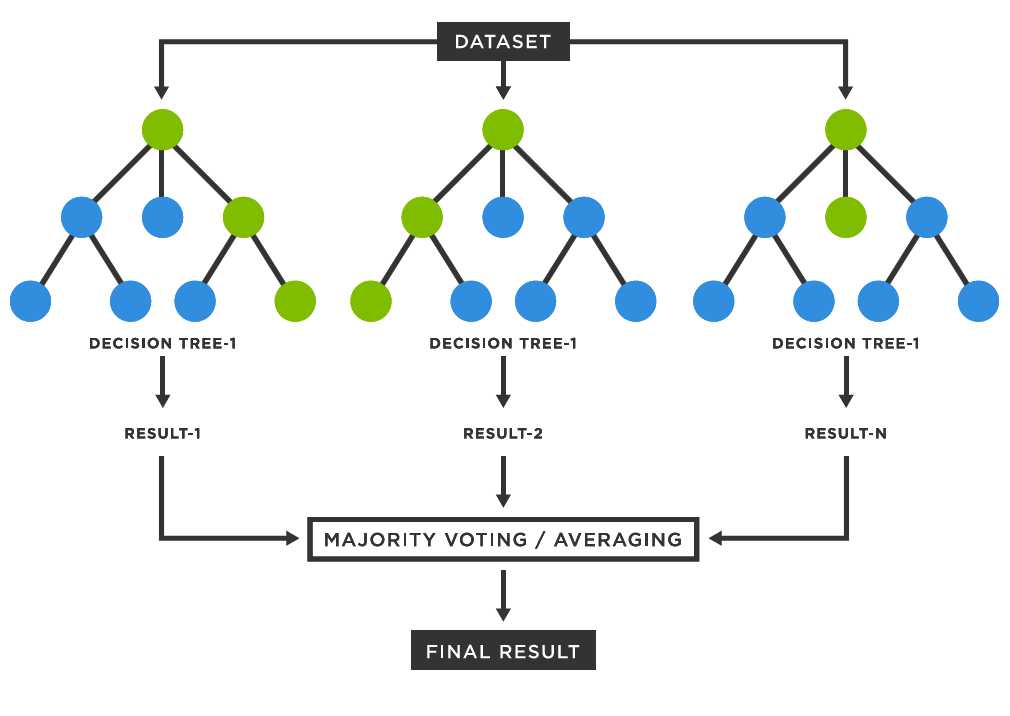
\includegraphics[width=0.75\linewidth]{images/randomForest.png}
    \caption{Illustration de la forêt aléatoire (\cite{gunay2023random})}
    \label{fig:fig5}
\end{figure}

\subsection{Implémentation}
\label{chap4.sec3.sub2}
Mon implémentation de la forêt aléatoire est conforme à l'agorithme \ref{chap4.sec3.sub1} avec deux légères différences (\cite{diarra2024notebooks}). Tout d'abord, le critère utilisé par les arbres de décisions pour choisir le prédicateur le plus important est différent du gain d'information. Pour cela j'ai utilisé le critère de l'impurété \textbf{gini} qui est une autre mésure de l’incertitude d’une variable aléatoire définie par la formule: \[Gini = 1 - \Sigma_i p_i^2\] où \(p_i\) est la probabilité de la classe \(i\). De manière similaire à l'entropie, une branche est pure si \(Gini = 0\), ce qui implique que le probabilité d'une classe est à 1 et toutes les autres à 0. Mais contrairement à l'entropie dont la valeur maximale est 1, le score gini le plus mauvais est de 0.5, signifiant que toutes les classes ont la même probabilité et donc que la branche est parfaitement hétérogène, par exemple dans notre cas avec deux classes: \(Gini_{max} = 1 - (0.5^2 + 0.5^2) = 0.5\). Le prédicateur le plus important est donc choisi comme celui avec le plus petit score gini. Le score gini a été choisi comme critère après avoir testé plusieurs mésures statistiques dont l'entropie et il s'est revélé être le plus rapide à calculer et donc le plus éfficace.

Ensuite, dans mon implémentation, les prédictions de la forêt sont retournées comme un vecteur représentant le probabilité de chacune des deux classes (fera défaut / ne fera pas défaut; représentés respectivement par 1 et 0), la classification de la forêt pour chaque exemple des données de test est obtenu en appliquant un seuillage sur la probabilité de la classe positive (1); seuil que j'ai fixé à 0,055 soit (5,5\%) pour maximiser la précision. Dans le chapitre 5 s'explique pourquoi ce seuil est si bas. La forêt est constituée de 200 arbres. Cet implémentation est basée sur celle de Scikit-learn (\cite{scikit-learn}).